\section{Description of the Model}
\subsection{Basic model: Hive simulation}
	Our model is widely based on the studies and equations of \textit{Khoury et al.} \cite{khoury13}. We used his quantitative models (equation~\ref{eq:changeBroodNumbers} to~\ref{eq:changeFoodStoreConst}) as described bellow and added new parameters to find out more about the bee's behaviour.\\
	Food, seasons, brood, foragers and hive bees are the cornerstone of our model. The dynamics of the hive is based on the bee's behaviour and their interaction with the environment as well as natural influences, i.e. seasons (which are separately added to \textit{Khoury's} model). Food here means nectar and pollen, which doesn't need to be further distinguished after according to \textit{Khoury} for simplicity reasons. After the queen laid an egg, a larvae develops inside a honeycomb cell. The equations show the proportionality of the brood to the food income and the relations between the bee number. Neglecting the complex process of reaching adulthood, we assume, according to \textit{Khoury} that larvae become adult hive bees 12 days after pupation. The mortality rate of hive bees or capped brood is negligible if there are not specific diseases implemented. The agents are only female bees, since they are responsible for maintenance and sustainability of the hive and foraging process. The males are ordinary hive bees. With all these information we can set up the equation for the brood number change:
	
	\begin{equation}\label{eq:changeBroodNumbers}
		{dB \over dt} = LS(H,f)-\phi B
	\end{equation}
	
	It associates different factors to the brood number. $L$ is rate of the bee queen and $S(H,f)$ is a function of the survival rate dependent on the amount of food and the number of hive bees. $\phi$ is the adult bee emerging factor and $B$ represents the uncapped brood. The equation gives us the survival rate of the brood $B$. $S(H,f)$ with $H$ representing the number of hive bees and $f$ the amount of food, is modelled as following:
	
	\begin{equation}\label{eq:functionHiveBeesFood}
		S(H,f)={f^2 \over f^2+b^2}{H \over H+v}
	\end{equation}
	
	The variable $v$ indicates the effect of the hive bees on the brood, whereas $b$ shows the food effect on brood survival. It decreases as food increases. As $f$ and $H$ become very large, $S(H,f)$ becomes constant. The first factor is a sigmoid function and shows the correlation of the food available and the capped brood. A decrease in brood can occur because of lack of food (they cannot be fed) and / or because adult bees consume the larvae to keep the resources in the hive and recycle the proteins (cannibalism). The second factor models the interdependency of the hive bee numbers on the survival of the brood. If there are large stores of food but no hive bees that can provide the food to the larvae, the brood survival also declines.  
	\\
	The second differential equation describes the rate at which the number of hive bees changes.	
	\begin{equation}\label{eq:changeHiveBees}
		{dH \over dt}=\phi B(t-\tau)-HR(H,F,f)
	\end{equation}
	
	$\tau$ is the ageing time and $\phi B(t-\tau)$ is the rate at which adult bees develop from pupation to adult bees (emergence rate). $H$ is again the hive bee number, the last term is the recruitment function and given as
		
		\begin{equation}\label{eq:recruitmentFunction}
			R(H,F,f) = \alpha_{min} + \alpha_{max}({b^2 \over b^2+f^2})-\sigma({F \over F+H})
		\end{equation}
				
	This function models the change from a hive bee to a forager bee. $\alpha_{min}$ denotes the transition when there is enough food but not much foragers. Vice versa, $\alpha_{max}$ is used for less food. As before, $b$ is the food effect on brood survival and $f$ is the amount of food. $\sigma$ is the strength of social inhibition and is dependent on the number of foragers and hive bees.\\
	The third differential equation describes correspondingly the rate at which the number of foragers changes:
	
	\begin{equation}\label{eq:changeForagers}
		{dF \over dt} = HR(H,F,f)-m F
	\end{equation}
	
	The mortality rate $mF$ indicated the rate at which the foragers $F$ die. The recruitment function is the same as above.\\	
	The last equation outlines with the rate of food change in the hive's stores. Forager bees and hive bees are treated equally because their consumption is almost the same. 
	
	\begin{equation}\label{eq:changeFoodStoreConst}
		{df \over dt} = c F - \gamma_A (F+H) - \gamma_B B
	\end{equation}
         
<<<<<<< HEAD
	where $c$ describes the average food a single forager collects per day. In our extended model, we also implemented a season dependent factor with the result that $c$ changes over time (see subsection~\ref{subsec:advancedModel} on page~\pageref{subsec:advancedModel}.). $\gamma$ is the consumption of adult bees ($A$) and brood ($B$).\\
	With those four differential equations, the change of brood (\ref{eq:changeBroodNumbers}), hive bee number (\ref{eq:changeHiveBees}), foragers (\ref{eq:changeForagers}) and change of food store (\ref{eq:changeFoodStoreConst}) and the functions of the brood survival rate, correlating to the hive bee number and the food store (\ref{eq:functionHiveBeesFood}) and a recruitment function (\ref{eq:recruitmentFunction}), we can simulate a basic model of a hive with its interactions and changes. So far, it is identical with \textit{Khoury's} model.
	
=======
	where $c$ describes the average food a single forager collects per day. $\gamma$ is the consumption of adult bees ($A$) and brood ($B$). In our extended model, we implemented an actual environment simulation so that the food income changes over time (see chapter \ref{chap:advancedModel}). Equation \ref{eq:changeFoodStoreConst} is then replaced by equation \ref{eq:changeFoodStoreDyn}, which takes the daily food income instead of a fixed rate $c$ per forager.

>>>>>>> 5eb25dfed511a52c6cb5f9bd3df977246b13b063
	\subsection{Changing laying rate over seasons}
		\begin{figure}
			\centering
			\scalebox{.75}{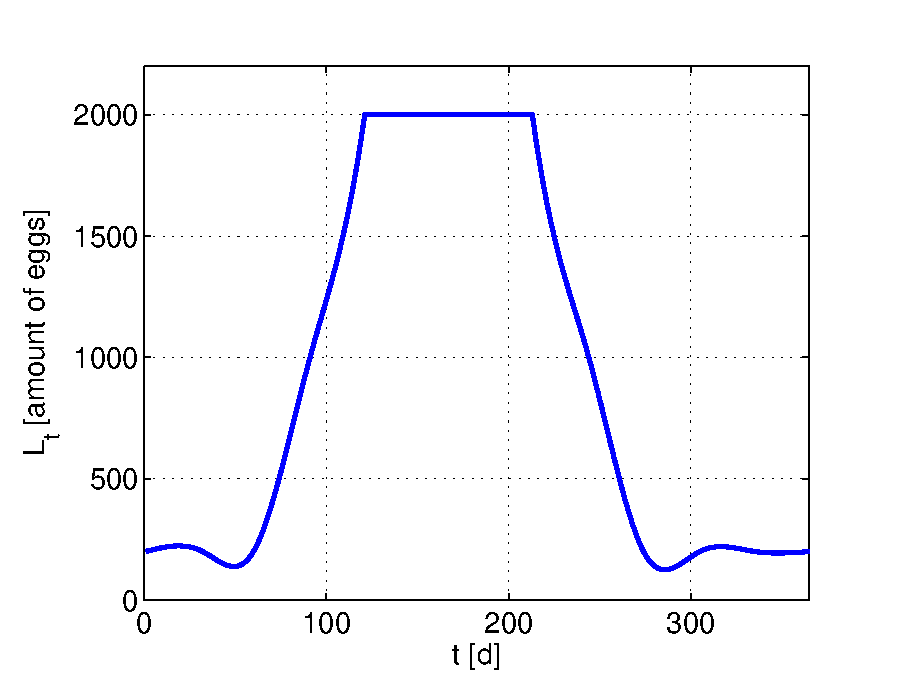
\includegraphics{data/egg_plot.eps}}
			\caption{\textit{The laying rate of the bee queen plotted over a year. The amount of eggs is capped after 2000 eggs. }}
			\label{fig:dynLayingRate}
		\end{figure}
		
<<<<<<< HEAD
		To make the model more realistic, equation \ref{eq:changeBroodNumbers} is replaced by equation \ref{eq:changeBroodNumbersTime}. This incorporates that the bee queen does not have a constant laying rate. Instead, interpolated values based on \textit{Wisdom of the Hive}, p. 34 \cite{seeley95} are used for the laying rate $L(t)$ (see fig.~\ref{fig:dynLayingRate}). \textit{T.D. Seeley} denotes that the queen starts reproducing by early spring. We assumed that reproduction between April/May and October is realistic, as we obtained similar numbers of bees in summer (maxima) and winter (minima) to the empirical data of \textit{T.D. Seeley} \cite{seeley95}. The minimal laying rate of 200 eggs per day is used to compensate mortality during winter. The peak of the laying rate (2000 eggs per day) is the same as used by \textit{Khoury et al.} \cite{khoury13} and \textit{Wright} \cite{wright08}. The results are discussed in chapters \ref{chap:constantFoodConstantLaying} and \ref{chap:constantFoodDynamicLaying} with the corresponding plots in appendix \ref{chap:sim_R0_1} and \ref{chap:sim_R0_2}.
=======
		To make the model more realistic, equation \ref{eq:changeBroodNumbers} is replaced by equation \ref{eq:changeBroodNumbersTime}. This incorporates that the bee queen does not have a constant laying rate. Instead, interpolated values based on \textit{Wisdom of the Hive}, pp. 34 \cite{seeley95} are used for the laying rate $L_t$ (Figure \ref{fig:dynLayingRate}). \textit{T.D. Seeley} denotes that the queen starts reproducing by early spring. We assumed that reproduction between April/May and October is realistic, as we obtained similar numbers of bees in summer (maxima) and winter (minima) to the empirical data of \textit{T.D. Seeley} \cite{seeley95}. The minimal laying rate of 200 eggs per day is used to compensate mortality during winter. The peak of the laying rate (2000 eggs per day) is the same as used by \textit{Khoury et al.} \cite{khoury13} and \textit{Wright} \cite{wright08}. The results are discussed in chapters \ref{chap:constantFoodConstantLaying} and \ref{chap:constantFoodDynamicLaying} with the corresponding plots in appendix \ref{chap:sim_R0_1} and \ref{chap:sim_R0_2}.
>>>>>>> 5eb25dfed511a52c6cb5f9bd3df977246b13b063
		
		\begin{equation}\label{eq:changeBroodNumbersTime}
			{dB \over dt} = L_tS(H,f)-\phi B
		\end{equation}
		
		%TODO: This belongs to the discussion section->
		The introduction of dynamic laying rates led to problems with the mortality rates tested by \textit{Khoury et al.} \cite{khoury13}. The colony we simulated did not survive with any daily mortality rates higher than 0.1. There are not enough bees emerging from eggs in order to compensate the mortality rate. However, we found that the new mortality rates assumed in our simulation (0.075 daily mortality) are still realistic. \textit{Henry et al.} \cite{henry12} describe mortality rates between 0.102 and 0.316 in empirical testing, which is the range in which \textit{Khoury et al.} \cite{khoury13} simulated. \textit{R. Dukas} \cite{dukas08} observed that mortality of foragers is in this range mainly because of predation. As we apply the mortality to all days, even in times and seasons without foraging (all bees stay in the hive), our simulated mortality rates are naturally lower.
	
	\subsection{Advanced model: Environment simulation}
		\label{chap:advancedModel}
		
% Define state styles
\tikzstyle{resource} = [circle, draw, top color=white, bottom color=red!20, draw=red!50!black!100, drop shadow, text width=1cm, text centered, node distance=2cm, minimum height=1cm]
\tikzstyle{bee} = [rectangle, draw, top color=white, bottom color=blue!30, draw=blue!50!black!100, drop shadow, text width=2cm, text centered, rounded corners, minimum height=1cm]
\tikzstyle{natural} = [rectangle, draw, top color=white, bottom color = green!30, draw=green!50!black!100, drop shadow, text width=2cm, text centered, rounded corners, minimum height=1cm]
\tikzstyle{line} = [line width=1.5pt, draw, -latex']


\begin{figure}[H]
	\centering
	\scalebox{0.6}{
	\large
	\begin{tikzpicture}[node distance = 3cm and 3cm, auto]
		% Place nodes
		\node [bee] (queen) {Queen};
		\node [bee, below of=queen, node distance = 2cm] (brood) {Uncapped brood};
		\node [bee, below of=brood, node distance = 2cm] (hiveBees) {Hive bees};
		\node [bee, below of=hiveBees, node distance = 2cm] (foragers) {Foragers and scouts};
		\node [resource, right of=brood, node distance = 5cm] (food) {Food};
		\node [natural, right of=food, node distance = 5cm] (environment) {Environment};
		\node [natural, below of=environment, node distance = 2cm] (flowers) {Flowers};
		\node [natural, above of=environment, node distance = 2cm] (seasons) {Seasons};
		% Draw edges
		\path [line] (queen.south) -- node {egg laying} (brood.north);
		\path [line] (brood.south) -- node {eclosion} (hiveBees.north);
		\path [line] ($(hiveBees.south)+(-0.25cm, 0.0cm)$) -- node [left] {food income requirements} ($(foragers.north)+(-0.25cm, 0.0cm)$);
		\path [line] ($(foragers.north)+(+0.25cm, 0.0cm)$) -- node [right] {social inhibition} ($(hiveBees.south)+(+0.25cm, 0.0cm)$);
		\path [line] (foragers.west) -- +(-1.0cm, 0.0cm) node [near end] {death};
		\path [line, dashed] (hiveBees.west) -- +(-0.5cm, 0.0cm) |-  node [near start] {affect survival} (brood.west);
		\path [line] (environment.north) -- node [left] {season durations}(seasons.south);
		\path [line] (environment.south) -- node [left] {patch distribution} (flowers.north);
		\path [line, dotted] (food) -- (queen.east);
		\path [line, dotted] (food) -- (hiveBees.east);
		\path [line, dotted] (food) -- (foragers.east);
		\path [line, dotted] (food) -- (brood.east);
		\path [line, dashed] (seasons.west) -- node {affect laying rate} (queen.east);
		\path [line, dashed] (seasons.east) -- +(0.5cm, 0.0cm) |- node [near start] {affect growth} (flowers.east);
		\path [line, dashed] (flowers.south) -- +(0.0cm, -2.5cm) node [above left] {foraging source availability} -| (foragers.south);
		\path [line, dotted] (foragers.east) -| node [near start, below] {food collection} (food.south);
	\end{tikzpicture}} 
	\caption{\textit{Honey bee social dynamics/influences covered by our model.}}
	\label{fig:modelOverview}
\end{figure}


<<<<<<< HEAD
		%TODO
		%TODO [This is actually wrong,] we did not change c in our (basic) model... have a look at the code. In the advanced model, we replace the term c * F with the result from the actual environment simulation! Please correct.
		(Food dependent on flowers\\
		In contrast to Khoury, we implemented also a seasonal dependent factor, so c changes with rate X over time. \\
		\\
		As we were interested in observing the social dynamics under different food availability conditions, in contrast to the model of 
		\\)
		\\
		Instead of just averaging the food source with an empirical value $c$, food collected per day, times $F$, forager count, we wanted to make it dependent on the environment. Equation \ref{eq:changeFoodStoreConst} changes to 
		
		\begin{equation}\label{eq:changeFoodStoreDyn}
			{df \over dt} = c_{dailySum}(t) - \gamma_A (F+H) - \gamma_B B
		\end{equation}
		
				
		 
		\subsubsection{Map and flower patches}
		%TODO
=======
		As we were interested in observing the social dynamics under different food availability conditions, in contrast to the model of \textit{Khoury et al.} \cite{khoury13}, we had to implement a simulation for the environment. This advanced model introduces an environment with seasons which affect the queen's laying rate (see equation \ref{eq:changeBroodNumbersTime}), the distribution and quality of flower patches and seasonal flower growth.
		The forager bees are then simulated on the environment, searching and collecting food according to the rules in chapter \ref{chap:beeWorkingStates}. An overview of the complete model is given in Figure \ref{fig:modelOverview}.
>>>>>>> 5eb25dfed511a52c6cb5f9bd3df977246b13b063
		
		\subsubsection{Bees' working states}
			\label{chap:beesWorkingStates}
			The environment simulation only simulates forager and scout bees. Hive bees are not considered as agents. For the foragers and scouts, we developed a set of simple rules which try to be as close as possible to the foraging process described by \textit{T.D. Seeley} \cite{seeley95}. All essential rules are represented in Figure \ref{fig:stateTransitionsEnvironment}.\\
			\label{chap:beeWorkingStates}
			
% Define state styles
\tikzstyle{decision} = [diamond, draw, top color=white, bottom color=red!20, draw=red!50!black!100, drop shadow, text width=4.5em, text badly centered, node distance=3cm, inner sep=0pt]
\tikzstyle{state} = [rectangle, draw, top color=white, bottom color=blue!30, draw=blue!50!black!100, drop shadow, text width=5em, text centered, rounded corners, minimum height=4em]
\tikzstyle{line} = [draw, -latex']


\begin{tikzpicture}[node distance = 2cm, auto]
	% Place nodes
	\node [state] (init) {initialize model};
	\node [cloud, left of=init] (expert) {expert};
	\node [cloud, right of=init] (system) {system};
	\node [state, below of=init] (identify) {identify candidate models};
	\node [state, below of=identify] (evaluate) {evaluate candidate models};
	\node [state, left of=evaluate, node distance=3cm] (update) {update model};
	\node [decision, below of=evaluate] (decide) {is best candidate better?};
	\node [state, below of=decide, node distance=3cm] (stop) {stop};
	% Draw edges
	\path [line] (init) -- (identify);
	\path [line] (identify) -- (evaluate);
	\path [line] (evaluate) -- (decide);
	\path [line] (decide) -| node [near start] {yes} (update);
	\path [line] (update) |- (identify);
	\path [line] (decide) -- node {no}(stop);
	\path [line,dashed] (expert) -- (init);
	\path [line,dashed] (system) -- (init);
	\path [line,dashed] (system) |- (evaluate);
\end{tikzpicture}



			
			At the beginning of every day ($t_s = 0$), all bees are unemployed. There are three possibilities for every unemployed bee which are considered in every simulation step:
			\begin{itemize}
				\item If the amount of active bees according to the current time of the day is not reached, the bee can get a job assigned. Otherwise the bee stays unemployed.
				\item If the maxima of scouts is not reached (6\% of the bees' foragers \cite*{seeley95}, p. 86), then the bee becomes a scout.
				\item Otherwise, the bee becomes a forager.\\
			\end{itemize}
			
			When a bee agent gets a scouting job assigned, the agent continues the following way:
			\begin{itemize}
				\item The scout performs a random walk (see chapter \ref{chap:randomWalk}) and checks with every iteration step, if any flower patch has been passed (see chapter \ref{chap:bresenhamAlgorithm}).
				\item If a flower patch is found or the flight distance limit is reached, the bee returns to the hive. Path optimization (see chapter \ref{chap:pathOptimization}) may occur.
				\item Back in the hive, the bee performs a waggle dance if scouting has been successful and goes back to the unemployed state.\\
			\end{itemize}
			
			When a bee agent gets a foraging job assigned, the agent continues the following way:
			\begin{itemize}
				\item Among the available waggle dances, the forager chooses randomly and evaluates if the food source is good enough ($p < q$) to visit or not (see chapter \ref{chap:foragersDistribution}). This is repeated in every iteration step until the forager decides to visit the flower patch represented by the chosen waggle dance.
				\item The forager flies to the patch and, once reached, collects as much food as the flowers in the patch allows (see chapter \ref{chap:mapFlowerPatchQuality}).
				\item After foraging, the bee returns to the hive. Path optimization may occur again.
				\item Back in the hive, the forager unloads the collected food (increasing $f_{d,t}$, equation \ref{eq:changeFoodStoreDyn}).
				\item The bee now has to evaluate the food source several times (($p < q$), once per iteration step) and decide if it is worth reporting the patch (executing a waggle dance) or not.
				\item A final evaluation ($p < q$) has to be done to decide if the forager will abandon it's own food source and become unemployed or fly to the same patch again.
			\end{itemize}
	
		
		\subsubsection{Foragers' distribution across flower patches}
			It is clear from chapter \ref{chap:beesWorkingStates} that after some time, the bees will focus on newly reported and then on the most profitable food sources because of relative quality evaluation. $p \in {[0,1]}$ denotes an equally distributed random value. $q$ denotes the relative quality of a given flower patch compared to all patches currently available as a waggle dance. In detail, the evaluation ($p < q$) works as follows:
			%TODO
		
		\label{chap:foragersDistribution}
		Depending on the random variable $p$ and the relative patch quality $q$ represented 
		
		
		\begin{equation}\label{eq:changeFoodStoreDyn}
			{df \over dt} = f_{d,t}- \gamma_A (F+H) - \gamma_B B
		\end{equation}
		Where $f_{d,t}$ denotes the amount of food the foragers collected on day $t$.
		
	\subsection{Empirical data bases}
<<<<<<< HEAD
		\subsubsection{Area around the hive}
			By analysing the different waggle dances of the forager bees, \textit{T.D. Seeley} states in \textit{Wisdom of the Hive} pp.~37ff that 95\% of the foraging process occurs in a radius of 6.0~km (maximum distance at 10.9~km, mean distance at 2.2~km and the modal distance at 1.6~km \cite{seeley95}. The approximation of our modelled square $(6~km * 2)^2 > (6~km)^2*\pi \approx 100~km^2$ should be sufficient for the simulation and comprehend all important data. In our model, we split the area up into a grid of 10~m~*~10~m tiles of flower patches.
		\subsubsection{Flower patches and food}
			The flower patches themselves are divided into their different blossom: spring, summer and autumn. The empirical data was taken from \textit{Wisdom of the Hive} p.~44 (year 1982) and the following page. We merged the raw data and received a new graph for the whole year (see fig.~\ref{fig:seasonalFlowers}). With equation \ref{eq:foodPerFlight}, we can find out the weight of food a bee carries per flight. 
			
			\begin{equation}\label{eq:foodPerFlight}
						w(t) [g/bee/flower] = \frac{M(t) \frac{kg}{d}}{C(t)}\cdot 1000 \frac{g}{kg}
			\end{equation}
			
			The result $w/t)$ is measured in gram per bee per flower. $M(t)$ is the mass change of the hive per day in kilograms.
			%TODO: isn't C(t) = F(t)?
			$M(t)$ denotes the change of the mass of the hive per day in kilograms (see fig.~\ref{fig:seasonalFlowers}) and $C(t)$ represents the forager bee count approximated for any day $t$ (\textit{T.D. Seeley's} empirical data \cite{seeley95}). Thus, we can take hive weight change per day as an indicator for the flower quality and flower type present at any given day of the year. 
			
			
				\begin{figure}
						\centering
						\scalebox{0.9}{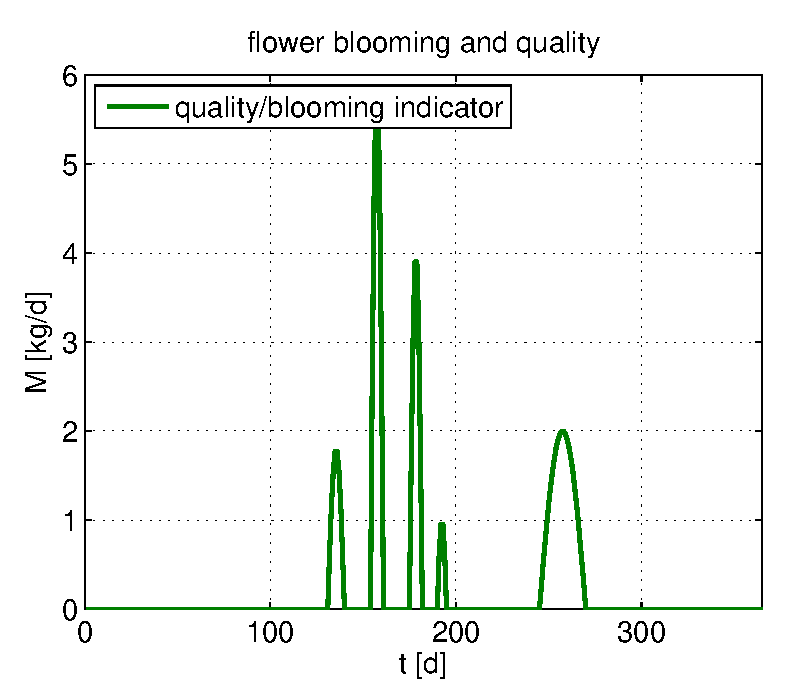
\includegraphics{data/seasonal_flowers.eps}}
						\caption{\textit{This figure shows the change of the mass of the hive for any day in the year. It correlates with the quality of a flower patch and the type of flower, respectively.}}
					\label{fig:seasonalFlowers}
					\end{figure}
=======
		By analysing the different waggle dances of the forager bees, \textit{T.D. Seeley} states in \textit{Wisdom of the Hive} pp.~37ff that 95\% of the foraging process occurs in a radius of 6.0~km (maximum distance at 10.9~km, mean distance at 2.2~km and the modal distance at 1.6~km \cite{seeley95} The approximation of $\text{(6~km}\cdot\text{2)}^2 \approx \text{100~km}^2$ should be sufficient for the simulation and comprehend all important data. In our model, we split the area up into a grid of 10~m~$\cdot$~10~m tiles of flower patches. \\
		The flower patches themselves are divided into their different blossom: spring, summer and autumn. The empirical data was taken from the \textit{Wisdom of the Hive} p.~44 (year 1982) and the following page. We merged the raw data and received a new graph for the whole year (see fig.~\ref{fig:seasonalFlowers}) The values are in hive weight change per kilogram per day. With equation \ref{eq:foodPerFlight}, we can find out the weight of food a bee can carry per flight.
		
		\begin{equation}\label{eq:foodPerFlight}
			\frac{M \frac{kg}{d}}{C}\cdot 1000 \frac{g}{kg} = Weight~per~bee~and~flower
		\end{equation}
		Where $M$ is a local certain height in the graph (Figure \ref{fig:seasonalFlowers}) and $C$ is the bee count of the hive approximated for day $t$ in \textit{T.D. Seeley's} empirical data \cite{seeley95}. Thus we can take hive weight change per day as an indicator for the flower quality and flower type present at any given day of the year. 
		
		
		\begin{figure}
			\centering
			\scalebox{0.9}{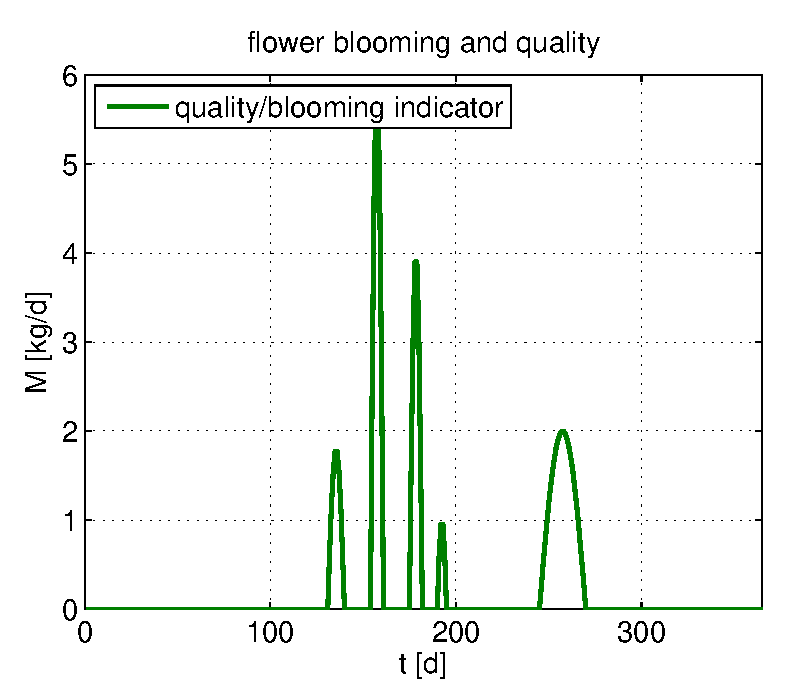
\includegraphics{data/seasonal_flowers.eps}}
			\caption{\textit{This figure shows flower blooming over a year. Well first it shows the UNnoramlized flower activity over a year. Second for the rest plz ask Fabian he did the Graph labeling all I can tell you is that it is a $1:1$ representation of the values from the Proberties\char`_Base file \ref{chap:MATLAB_Base}~$Prop.Sim.Flower.peak \cdot Prop.Sim.Flower.year\char`_activity$ }}
			\label{fig:seasonalFlowers}
		\end{figure}
>>>>>>> 5eb25dfed511a52c6cb5f9bd3df977246b13b063
	
	%TODO
		\subsubsection{Different kinds of bees and their behaviour}
			
		
	%-Why is it 470 days?
%	-bee count 10'000? why? 
%	-hive bees 16000
%	-foragers 8000
%	-food_brood_eff = 500;
%	-hive_brood_eff = 5000;
%	-aging_time = 12
%	-mortality = 0.075 (see above)
%	-min recruitment 0.25
%	-max rec 0.25
%	-laying rate in winter -> to keep hive alive
%	-social inhibition (<=!=> recruitment)
%	-adult bee emerging 1/9
%	-food = 50000
%	-food_consumption_adult = 0.007
%	-food_consumption_brood = 0.018
%	-Barrier for extinction. If total bee count is lower than this, a hive is considered extinct (no more computation, all values constant and/or zero) extinct_barrier = 500;
%	 
	
